\documentclass[11pt]{article}
\usepackage{graphicx}
\usepackage{listings}
\usepackage{xcolor}
\usepackage{hyperref}
\usepackage[margin=1in]{geometry}
\usepackage{bugtracker} % Ajusta los márgenes a 1 pulgada
\definecolor{codegreen}{rgb}{0,0.6,0}
\definecolor{codegray}{rgb}{0.5,0.5,0.5}
\definecolor{codepurple}{rgb}{0.58,0,0.82}
\definecolor{backcolour}{rgb}{0.95,0.95,0.92}

\lstdefinestyle{mystyle}{
    backgroundcolor=\color{backcolour},
    commentstyle=\color{codegreen},
    keywordstyle=\color{magenta},
    numberstyle=\tiny\color{codegray},
    stringstyle=\color{codepurple},
    basicstyle=\ttfamily\small,
    breakatwhitespace=false,
    breaklines=true,
    captionpos=b,
    keepspaces=true,
    numbers=left,
    numbersep=5pt,
    showspaces=false,
    showstringspaces=false,
    showtabs=false,
    tabsize=2
}

\lstset{style=mystyle}

\title{Informe sobre Umbralización por Histéresis}

\author{RUBEN MARTINEZ GONZALEZ}
\date{\today}

\begin{document}

    \maketitle
    \begin{center}
        \textbf{Visión computacional}
    \end{center}


    \section{Introducción}
    \noindent
    En este informe, se presenta la adaptación realizada para implementar la umbralización por histéresis.
    \noindent
    La solución se implementó en Python y está desplegada en un notebook de Google Colab, el cual se puede acceder a través del siguiente enlace:
    \texttt{%
        \href{https://colab.research.google.com/drive/1jJnkRD_QYszGcF4tEZ0V2oYQkkZl8hcF?usp=sharing}{%
            Colab}%
    }


    \section{Umbralización por histéresis}
    La umbralización por histéresis es una técnica utilizada en el procesamiento de imágenes para detectar bordes.
    Se basa en el uso de dos umbrales: uno alto y otro bajo.
    Los píxeles que están por encima del umbral alto se consideran como píxeles de borde fuertes, mientras que los píxeles que están por encima
    del umbral bajo pero por debajo del umbral alto se consideran como píxeles de borde débiles. Los píxeles por debajo del umbral bajo se descartan.


    \section{Adaptación del Algoritmo}
    Para adaptar el algoritmo de búsqueda en profundidad para realizar la umbralización por histéresis, realizamos las siguientes modificaciones:
    \begin{itemize}
        \item Parámetros de umbralización: En la función busca(), se agregaron dos nuevos parámetros low\_threshold y high\_threshold para representar
        los umbrales de intensidad inferior y superior, respectivamente.
        \item Condiciones de etiquetado: En lugar de simplemente etiquetar los píxeles como conectados o no conectados, ahora se verifica
        si el valor de intensidad del píxel está dentro del rango especificado por los umbrales. Si el valor del píxel cumple con esta condición,
        entonces se etiqueta con el valor fijo de 255. Si no cumple con la condición, se descarta y no se etiqueta por lo que se mantendra con valor 0.
        \item Llamada recursiva condicional: Dentro de la función busca(), la llamada recursiva ahora se realiza solo si el valor de intensidad del píxel vecino
        está dentro del rango de los umbrales especificados.
        \item Función de etiquetado adaptada: La función de etiquetado principal etiqueta\_con\_umbralizacion() ahora toma en cuenta los umbrales de intensidad al llamar a busca().
    \end{itemize}

    \begin{lstlisting}[language=Python, caption=Función de Umbralización por Histéresis en Python]
def busca_con_umbralizacion(I, E, i, j, b, low_threshold, high_threshold):
    if low_threshold <= I[i, j] <= high_threshold:
        E[i, j] = b
        for k in range(-1, 2):
            r = k + i
            if r < 0 or r >= I.shape[0]:
                continue
            for l in range(-1, 2):
                if k == 0 and l == 0: continue
                c = l + j
                if c < 0 or c >= I.shape[1]: continue
                if low_threshold <= I[r, c] <= high_threshold
                and E[r, c] == 0:
                    busca_con_umbralizacion(I, E, r, c, b,
                             low_threshold, high_threshold)

def etiqueta_con_umbralizacion(I, low_threshold, high_threshold):
    E = np.zeros(I.shape)
    b = 255
    for i in range(I.shape[0]):
        for j in range(I.shape[1]):
            if I[i, j] >= high_threshold and E[i, j] == 0:
                busca_con_umbralizacion(I, E, i, j, b, low_threshold, high_threshold)
    return E
    \end{lstlisting}


    \section{Resultado}
    En el ejemplo de uso, se define una imagen con valores en el rango de 0 a 255 y se especifican los umbrales low\_threshold y high\_threshold.
    Luego, se llama a la función etiqueta\_con\_umbralizacion() con estos parámetros.
    \begin{lstlisting}[language=Python, caption=Ejemplo de Uso]
image = np.array([
    [99, 255, 255, 255, 0, 0, 0, 99],
    [99, 255, 255, 255, 0, 0, 0, 99],
    [99, 255, 255, 255, 0, 0, 0, 99],
    [99, 99, 99, 99, 99, 99, 99, 99],
    [99, 0, 0, 0, 255, 255, 255, 99],
    [99, 0, 0, 0, 255, 255, 255, 99],
    [99, 0, 0, 0, 255, 255, 255, 99],
])

# Definir umbrales de intensidad
low_threshold = 100
high_threshold = 255

# Etiquetar los componentes conectados en la imagen con umbralización
E = etiqueta_con_umbralizacion(image, low_threshold, high_threshold)
    \end{lstlisting}

    \begin{figure}[htbp]
        \centering
        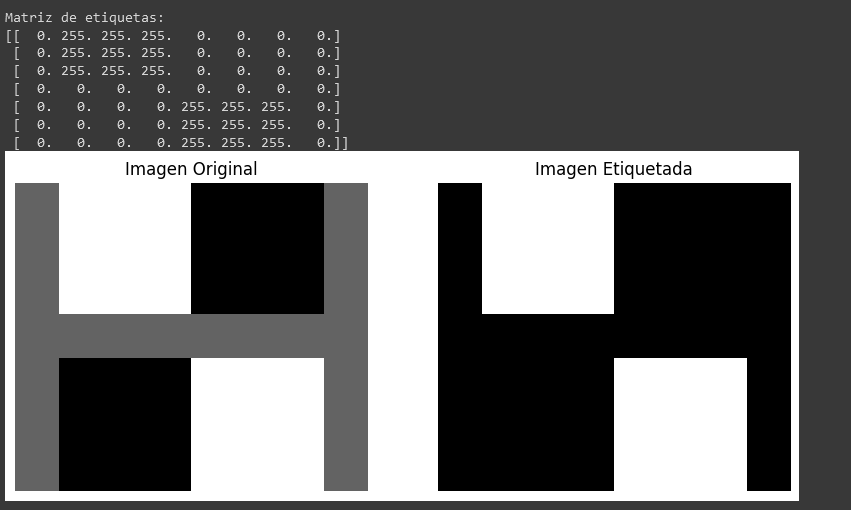
\includegraphics[width=0.99\textwidth]{resultado_umbralizacion_histéresis.png}
        \caption{Resultado de la Umbralización por Histéresis}
        \label{fig:resultado}
    \end{figure}

\end{document}
